\documentclass[a4paper,12pt]{article}

% very small margins (around 1.5cm)
% disable package geometry if you use this
\usepackage{fullpage}

% some mathematical symbols
\usepackage{amsmath}

% mathematical symbols
% conflicts with package program
\usepackage{amssymb}

% url addresses using \url{http://domain.com/}
\usepackage{url}

% use \includegraphics[scale=1.00]{file.jpg} for images
\usepackage{graphicx}

% for proper placement of floating figures
\usepackage{float}

\usepackage{multirow}
%\usepackage{pseudocode}
%\usepackage{booktabs}
%\usepackage{color}
%\usepackage{algorithmic} %pseudocode
%\usepackage{algorithm} %pseudocode as whole procedures
%\usepackage{program} %more sophisticated pseudocode

% use \begin{comment} ... \end{comment} for multiline comments
\usepackage{comment}

\begin{document}

\title{Static fluid~flow~simulation using~the~finite~element~method}
\date{January 28, 2014}
\author{Mateusz Bysiek, Computer Science A/S, MiNI, WUT}
\maketitle

\begin{footnotesize}

This is thoretical background for the project realized as part of ``From finite~element~method to signal analysis'' course at Computer~Science,
Faculty~of~Mathematics~and~Information~Science, Warsaw~University~of~Technology.

\end{footnotesize}

\section{Task}

Write a computer program that implements finite element method for static fluid flow, for uniorm triangular and
rectangular meshes. Use Laplace's equation.

\section{Theoretical background}

It is important to note that:

\begin{itemize}

  \item the static fluid flow problem is a problem completely different from the dynamic fluid flow problem, and this
  solution does apply only to static fluid flow problem;

  \item also, this solution is only a very simplified model of reality; and

  \item at this project's level, the task of static fluid flow simulation is equivalent to static heat transfer
  simulation (more about that later on).

\end{itemize}

It seems more intuitive to talk about the static heat transfer, than about static fluid flow, and for that reason I shall
start with example related to heat transfer.

\subsection{Static heat transfer}

When we talk about static heat transfer, it can be understood as how the temperature will be distributed across space
given some initial conditions. \cite{wiki_heat_transfer}

\newpage

Let us consider a following example.

We have a generally ``neutral'' environment, for example some place few meters underground. Plus, we have some
relatively hot places in our environment. They can be any source of heat, for example some pipes with hot water. Also,
we have some relatively cold places in our environment. They can be any hypothetical devices that suck in heat, or just
some pipes with coolant, or cold water. What characterizes such environment is that it is static -- the water in the
pipes always has the same temperature.

\begin{figure}[H]
\begin{center}
  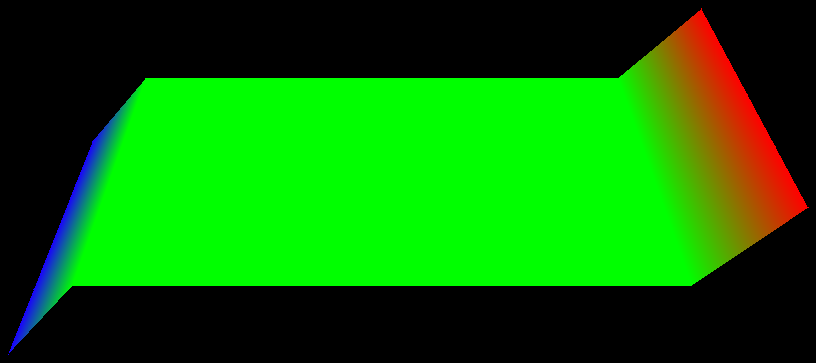
\includegraphics[width=\textwidth]{heat_before}
\end{center}
\caption{green is a neutral environment, red and high is a pipe with hot water, blue and low is a pipe with cold water}
\end{figure}

Using static flow calculations, we can predict exaclty what temperature will be at each point in our environment. You
may notice, that normally such predictions would require you to make calculations for each point, and since heat
propagates in the ground, after you calculate temperature at some point you have to adjust temperature at all
neighbouring points. This leads to either infinite calculations, or if you know how to handle such problems it leads to
partial differential equations.

Differential equations are solvable, but first of all are complicated, so they require large computational power. Second
of all, you rarely need to know exact temperature in every place around. Usually some regions are of more interest than
others, and more importantly, even in these regions you probably don't need to know the temperature at every single
point.

\newpage

And that is where the finite element method comes in. For example, for you may want to know the approximate temperature
of every $m^2$ of the ground. You can divide your whole environment into fragments called \emph{elements}. In our
example, you may call each square meter the \emph{element}. \cite{wiki_finite_element_method}

\begin{figure}[H]
\begin{center}
  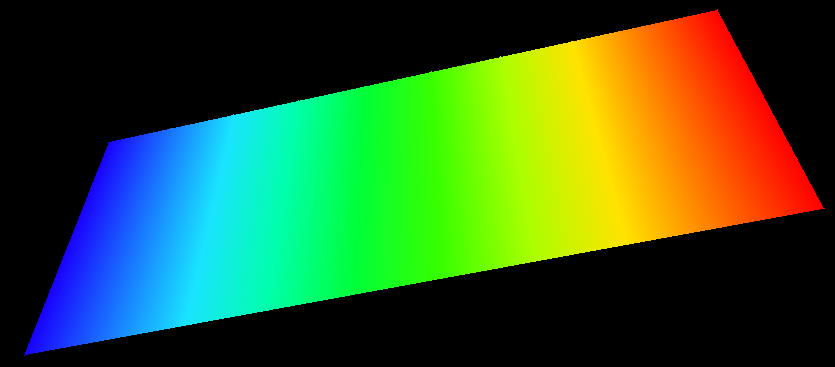
\includegraphics[width=\textwidth]{heat_after}
\end{center}
\caption{instant result, after appying the finite element method}
\end{figure}

We can divide the space into rectangular elements of any size, and by choosing the size we can adjust precision of our
result, as well as how much time we spend on computation. If we assume that area under consideration is a rectangle of
ground of size $9$ by $4$ meters, we have $36m^2$ in total, and therefore 36 elements.

\begin{figure}[H]
\begin{center}
  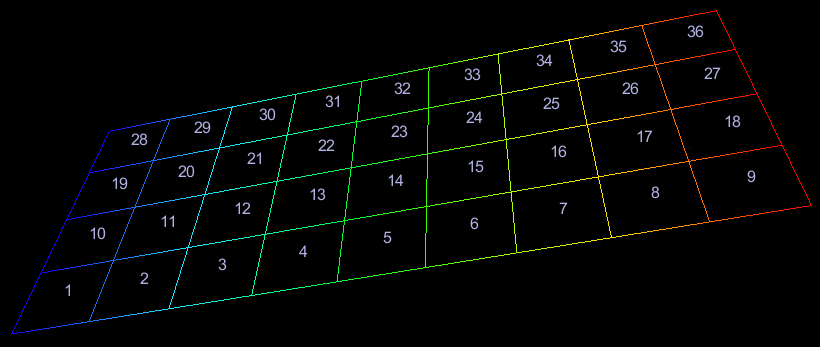
\includegraphics[width=\textwidth]{heat_elements}
\end{center}
\caption{labeled elements from the above example}
\end{figure}

\newpage

\subsection{Static fluid flow}

Static fluid flow can be understood as the potential of how the water will flow given some initial conditions.

(\ldots)

%\begin{comment}

For example we have something like this:

\begin{figure}[H]
\begin{center}
  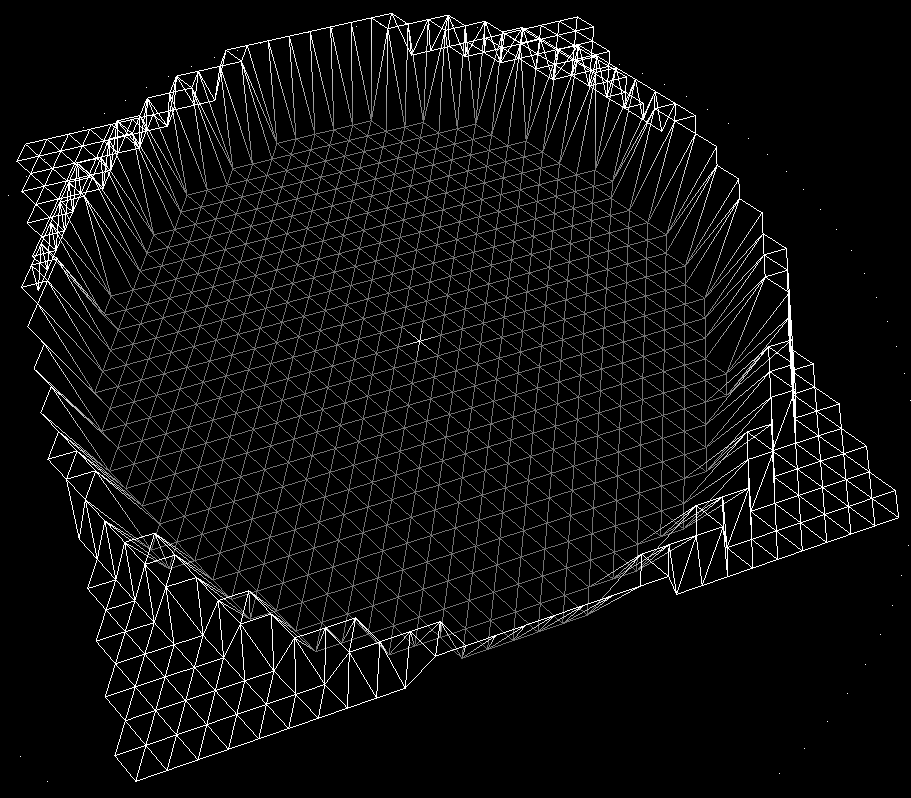
\includegraphics[width=\textwidth]{flow_initial}
\end{center}
\caption{initial conditions, white are fixed/known values, grey are the unknown}
\end{figure}

What can it be? Let's consider what happens when you put sugar into your tea, you get a spoon and start stirring. Now,
you want to know how the surface of your tea behaves while you do that. You know that the middle point is still, more or
less. You also know that the circular border close to your cup is moving at some speed which is the same around your cup.

The middle point and the border are shown in white because we assume that these values are constant. Around the centre
we have some grey area where we don't know how the fluid behaves. It's important to remark that the height of each point
shows not the physical height, but rather corresponds to speed at which the fluid is moving at that point. The grey
surface in the middle is your tea, as well as the white point in the middle, as well as the high circle. Let us not
consider corners, as they represent some area outside the cup.

Calculating exact velocity of each point requires calculation of velocity at nearby points. We would have quickly become
overwhelmed by such calculations, but, as in case of heat, we fortunately can divide the space into elements, this time
let them be triangular elements.

\begin{figure}[H]
\begin{center}
  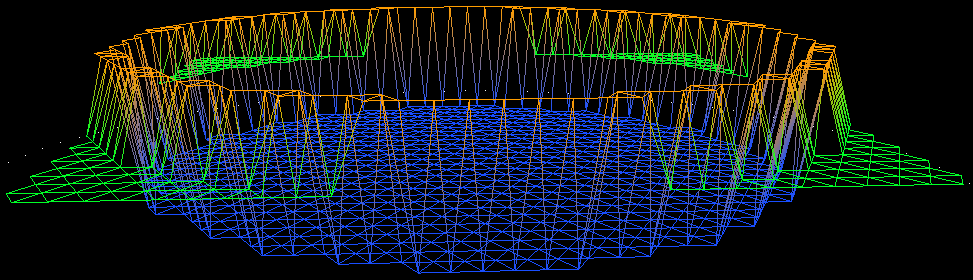
\includegraphics[width=\textwidth]{flow_before}
\end{center}
\caption{initial conditions, blue is slow, orange is fast}
\end{figure}

\begin{figure}[H]
\begin{center}
  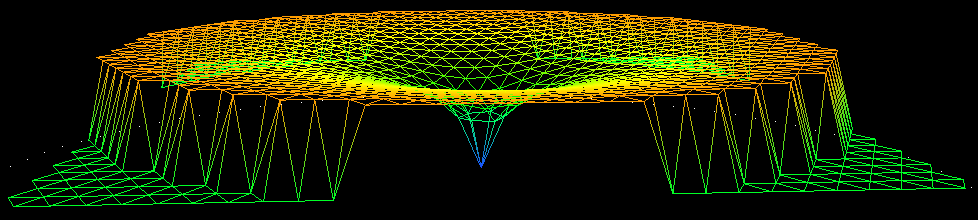
\includegraphics[width=\textwidth]{flow_after}
\end{center}
\caption{results after using finite element method}
\end{figure}

Is this the correct solution for such problem? Once again, what you can see here is not how high the surface of a fluid
is, but rather how fast it moves. But even after considering this, you can see that even if in the middle the fluid is
completely still, very near to this central point it moves quite fast. If you take a close look at real stirred tea, it
is quite different.

%We can actually calculate that since the angular speed of 

This is because there are some great simplifications in the used method. For example, in this model, we assume that
there is no viscosity, and also, that the particles of the fluid do not rotate. In case of stirring tea the second
condition is broken. If we would have stirred honey instead of tea, we would fail to fulfill both conditions, because
even if we may neglect viscosity of water, we certainly shouldn't neglect viscosity of honey.

%\end{comment}

\subsection{Laplace's equation}

From theoretical point of view, if you wish to determine how fast fluid flows at each location, or if you wish to
determine what temperature is at each location -- after simplification it is the same problem. And to solve it is the
same as to solve the Laplace's equation for given conditions. \cite{wiki_laplaces_equation}

\[ \Delta \phi =  \nabla^2 \phi = 0 \]

Specifically, in 2 dimensions the equation has a certain form.

\[ \frac{\partial^2 \psi}{\partial x^2} + \frac{\partial^2 \psi}{\partial y^2} \equiv \psi_{xx} + \psi_{yy} = 0 \]

%This means that our problem is a very specific case, and even partial differential equations are simplified.

\subsubsection{Triangular elements}

Trianglar elements are those that have 3 vertices. In this solution, I assume that all triangles have the same size. It
is important to remark that size is calculated using only two dimensions, as the third dimension is not really
``height'' but rather value of the function based on two values.

\begin{figure}[H]
\begin{center}
  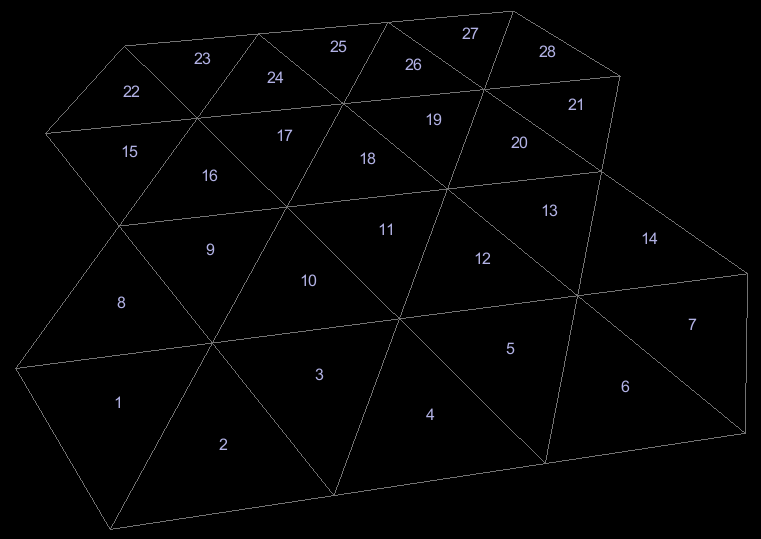
\includegraphics[width=\textwidth]{mesh_triangular}
\end{center}
\caption{a mesh consisting of triangular elements}
\end{figure}

%(\ldots)

\subsubsection{Rectangular elements}

Rectangular elements are those that have 4 vertices. In this solution, I assume that all rectangles are of the
same size. As in case of triangular elements, it is important to remember the method of calculating the size.

\begin{figure}[H]
\begin{center}
  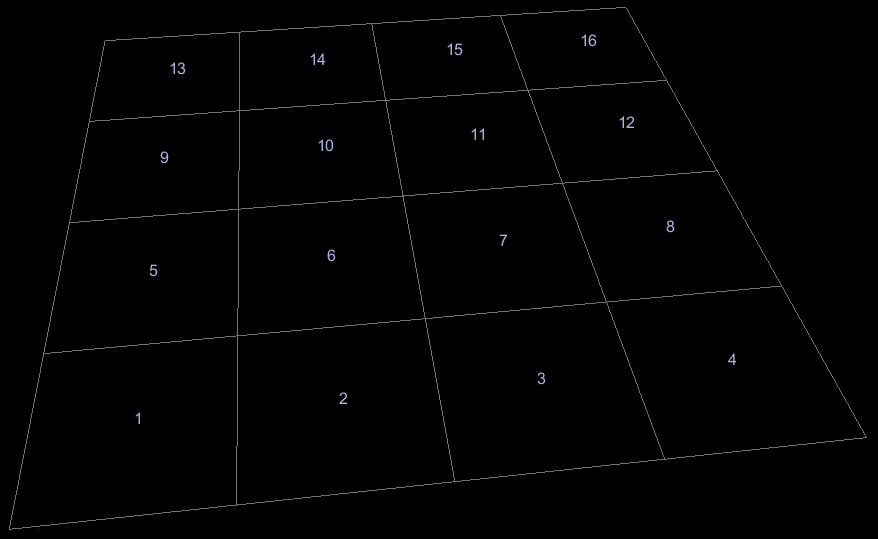
\includegraphics[width=\textwidth]{mesh_rectangular}
\end{center}
\caption{a mesh consisting of rectangular elements}
\end{figure}

%(\ldots)

\section{Implementation}

Computational part is implemented in C++, user interface is made using Qt, while the visualization itself is made using
OpenGL.

\subsection{Technologies}

The FEM computations are implemented in C++11. Full list of technologies used for computation:

\begin{itemize}
  \item C++11 -- backbone of the implementation
  \item Boost uBLAS (Basic Linear Algebra Library) -- part of Boost dedicated to linear algebra and matrix operations
\end{itemize}

The visual part of the solution is implemented using OpenGL. Full list of technologies used for visualization:

\begin{itemize}
  \item Qt -- for GUI (Graphical User Interface)
  \item OpenGL -- backbone of 3D visualization
  \item freetype -- for FreeType fonts displayed in OpenGL environment
  \item ftgl -- for displaying text in OpenGL environment.
\end{itemize}

Other general-purpose technologies used:

\begin{itemize}
  \item Doxygen -- for technical documentation
  \item LaTeX -- for theoretical documentation and user guide
  \item libxml2 -- for file I/O
\end{itemize}

\subsection{Algorithm}

The program starts with measuring the most important parameters of the mesh:

\begin{itemize}

  \item Number of vertices in mesh is $N$.

  \item Total number of elements (i.e. triangles or rectangles) is $E$.

  \item Number of vertices in each element of the mesh is $V$ -- for triangular elements $V$ is $3$, for rectangular it
  is $4$.

  \item Number of vertices that have defined boundary condition is $B$.

\end{itemize}

Three main matrices are creates:

\begin{itemize}

  \item A stiffness matrix $S$, of size $N \times N$.

  \item A mass matrix $M$, of size $1 \times N$ -- in other words a $N$-dimensional vector.

  \item A result matrix $R$, of size $1 \times N$

\end{itemize}

All of the values in matrices $S$ and $M$ are set to zero.

Then, a supporting matrix, local stiffness matrix $L$ of size $V \times V$ is created.

$L$ is set to precalculated results of two-dimensional integration so that for each element the correct ``shape'' of
importance of each vertex is applied.

\begin{itemize}

  \item For triangulr elements:
  \[
  \left| \begin{array}{rrr}
  %\left[ \begin{aligned}
  -0.18 &  0.09 &  0.09 \\
   0.09 & -0.17 &  0.08 \\
   0.09 &  0.08 & -0.17 \\
  %\end{aligned} \right]
  \end{array} \right|
  \]

  \item For rectangular elements:
  \[
  \left| \begin{array}{rrrr}
   0.666667 & -0.166667 & -0.333333 & -0.166667 \\
  -0.166667 &  0.666667 & -0.166667 & -0.333333 \\
  -0.333333 & -0.166667 &  0.666667 & -0.166667 \\
  -0.166667 & -0.333333 & -0.166667 &  0.666667 \\
  \end{array} \right|
  \]

\end{itemize}

After that, iteration over all $E$ elements starts. For each element the same below procedure is repeated:

\begin{itemize}

  \item a ``multiplier'' is calculated from the determinant of the element. That ``multipier'' depends directly on the
  area of the element, i.e. if all elements of the mesh have the same size, all ``multipliers'' are identical.

  \item to the stiffnes matrix $S$, the partial results of $L$ times the ``multiplier'' are added.

\end{itemize}

Then, iteration over all $B$ vertices that have boundary condition starts. For each such point the following is done:

\begin{itemize}

  \item Each vertex has a corresponding row of the stiffness matrix $S$, since height of $S$ is equal to $N$. The row
  that corresponds to current $i$th boundary-conditioned vertex is set to the vector$(0,\ldots,1,\ldots,0)$ where the
  $1$ is placed at $i$th place. Incidentally it is on the diagonal of the stiffness matrix.
  
  \item Each such vertex also has a corresponding element of of mass matrix $M$, since its height is also equal to $N$.
  The value at $i$th place of $M$ is set to the boundary condition (i.e. the ``z'' coordinate of the vetrex).

\end{itemize}

At this point, the stiffness matrix $S$ and mass matrix $M$ are both ready, and the resulting matrix $R$ is calculated
by left division of $S$ by $M$.

\section{Examples}

\subsection{Trivial}

In the trivial case, where there are no conditions defined at all, the software is behaving nicely by not altering the
input with any noise.

\subsection{Bounary conditions}

If the whole border of the mesh has defined boundary conditions, the software of course manages to compute the final
result. For small mesh sizes (up to approx. 15 x 15) the computation happens in real-time.

\subsection{Free boundaries}

The program manages to compute correctly in situations where some part of border has no boundary conditions.

For example:

\begin{figure}[H]
\begin{center}
  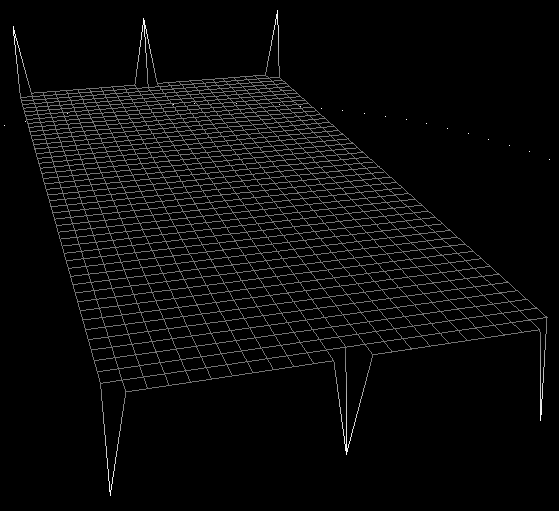
\includegraphics[width=\textwidth]{six_points}
\end{center}
\caption{here, only 6 points are defined as boundary conditions, in white colour; the rest is grey, meaning undefined}
\end{figure}

\begin{figure}[H]
\begin{center}
  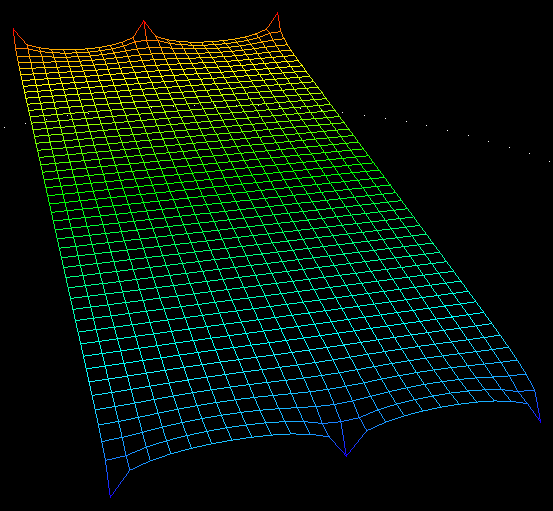
\includegraphics[width=\textwidth]{six_points_smooth}
\end{center}
\caption{after appying the finite element method}
\end{figure}

%\subsection{Several other examples}

%I would like to include some nice examples of smoothened planes, which in the end inspired the name of the application. 

\begin{thebibliography}{9}

\bibitem{wiki_heat_transfer}
  Heat transfer,
  Wikipedia,
  \url{https://en.wikipedia.org/wiki/Heat_transfer},
  accessed 2014-01-22

\bibitem{wiki_fluid_statics}
  Fluid statics,
  Wikipedia,
  \url{https://en.wikipedia.org/wiki/Fluid_statics},
  accessed 2014-01-22

\bibitem{wiki_finite_element_method}
  Finite element method,
  Wikipedia,
  \url{https://en.wikipedia.org/wiki/Finite_element_method},
  accessed 2014-01-22

\bibitem{wiki_laplaces_equation}
  Laplace's equation,
  Wikipedia,
  \url{https://en.wikipedia.org/wiki/Laplace's_equation},
  accessed 2014-01-22

\bibitem{wiki_stiff_equation}
  Stiff equation,
  Wikipedia,
  \url{https://en.wikipedia.org/wiki/Stiff_equation},
  accessed 2014-01-22

\bibitem{wiki_stiffness_matrix}
  Stiffness matrix,
  Wikipedia,
  \url{https://en.wikipedia.org/wiki/Stiffness_matrix},
  accessed 2014-01-22

\bibitem{wiki_mass_matrix}
  Mass matrix,
  Wikipedia,
  \url{https://en.wikipedia.org/wiki/Mass_matrix},
  accessed 2014-01-22

\bibitem{wiki_matrix_division}
  Division of matrices,
  Wikipedia,
  \url{https://en.wikipedia.org/wiki/Division_\%28mathematics\%29#Of_matrices},
  accessed 2014-01-22

\bibitem{laplaces_equation}
  Laplace Equaion,
  The Engineering ToolBox,
  \url{http://www.engineeringtoolbox.com/laplace-equation-d_622.html},
  accessed 2014-01-28

\bibitem{wiki_}
  Potential Flow Theory,
  MIT Open Courseware,
  \url{http://ocw.mit.edu/courses/mechanical-engineering/2-016-hydrodynamics-13-012-fall-2005/readings/2005reading4.pdf},
  accessed 2014-01-28

\end{thebibliography}

\end{document}
